\section{Introdução à hidráulica}

\begin{frame}{Introdução}
	\begin{block}{}
		\begin{itemize}
			\item A hidráulica é muito similar a pneumática porém, por usar \textbf{líquidos}, ou seja, fluidos \textbf{incompressíveis}, acaba tendo uma enorme vantagem sobre a pneumática, já que pode operar com forças \textbf{muito maiores}.
			\item As prensas hidráulicas chegam a \textbf{100 toneladas} de força facilmente.
		\end{itemize}
	\end{block}
	
	\centering
	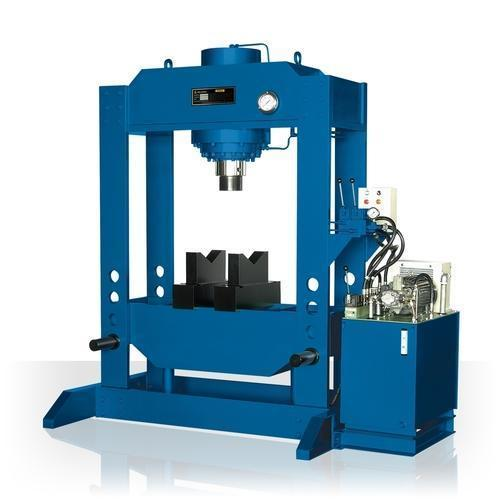
\includegraphics[width=0.45\linewidth]{Figuras/Ch15/fig1}

\end{frame}


\begin{frame}{Princípios físicos}
	\begin{block}{Introdução}
		Além dos princípios estudados anteriormente, que governam o movimento, pressão e força dos fluidos, existe o \textbf{princípio de Pascal} que é \textbf{essencial }na hidráulica.
	\end{block}

	\medskip
	
	\centering
	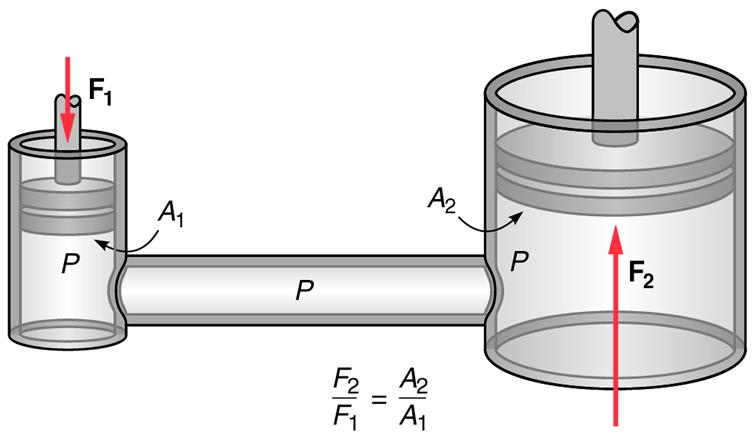
\includegraphics[width=0.7\linewidth]{Figuras/Ch15/fig6}
	
\end{frame}


\begin{frame}{Princípios físicos}
	\begin{block}{Lei de Pascal}
		\begin{itemize}
			\item A lei de Pascal nos diz que a pressão exercida em um ponto qualquer de um fluido estático é \textbf{a mesma} em \textbf{todas as direções}, exercendo \textbf{forças iguais} em \textbf{áreas iguais}.
		\end{itemize}
	\end{block}
	
	\centering
	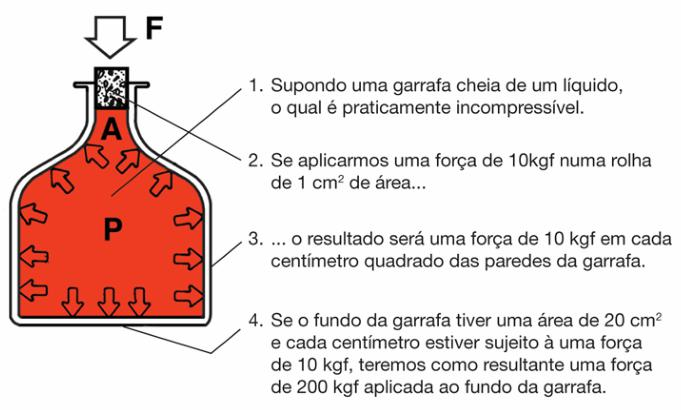
\includegraphics[width=0.7\linewidth]{Figuras/Ch15/fig2}
	
\end{frame}


\begin{frame}{Princípios físicos}
	\begin{block}{Lei de Pascal}
		\begin{itemize}
			\item Esse princípio se estende para nos dar um resultado muito útil: \textbf{a prensa hidráulica}.
		\end{itemize}
	\end{block}
	
	\centering
	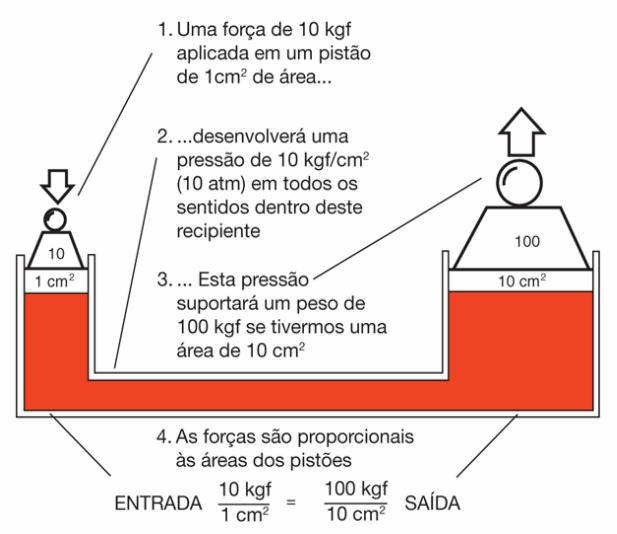
\includegraphics[width=0.55\linewidth]{Figuras/Ch15/fig3}
	
\end{frame}


\begin{frame}{Princípios físicos}
	\begin{block}{Lei de Pascal}
		\begin{itemize}
			\item Repare que as quantidades ainda são conservadas: nenhuma lei física foi desobedecida aqui.
		\end{itemize}
	\end{block}
	
	\centering
	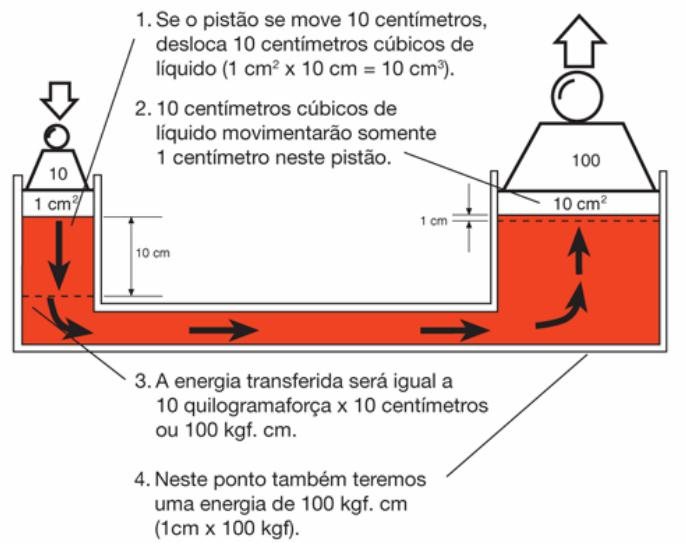
\includegraphics[width=0.6\linewidth]{Figuras/Ch15/fig4}
	
\end{frame}


\begin{frame}{Sistema hidráulico básico}
	\begin{block}{Introdução}
		Na hidráulica é necessário esquematizar um sistema fechado em \textbf{\textit{loop}}, já que \textbf{não é possível despejar} o fluido usado no sistema em qualquer lugar, e nem é fácil arranjar mais para uso.
	\end{block}
	
	\medskip
	\centering
	
	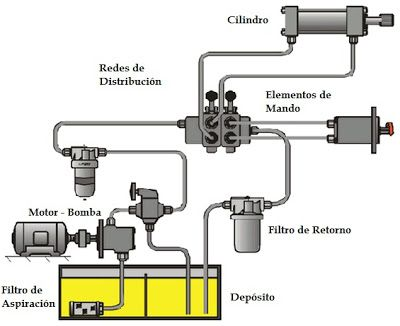
\includegraphics[width=0.5\linewidth]{Figuras/Ch15/fig5n2}
	
\end{frame}


\begin{frame}{Sistema hidráulico básico}
	\begin{block}{}
		No diagrama hidráulico básico temos:
		\begin{itemize}
			\item Fonte de energia.
			\item Grupo de geração.
			\item Grupo de controle.
			\item Grupo de atuação.
			\item Grupo de ligação.
		\end{itemize}
	\end{block}

	\medskip
	\centering
	
	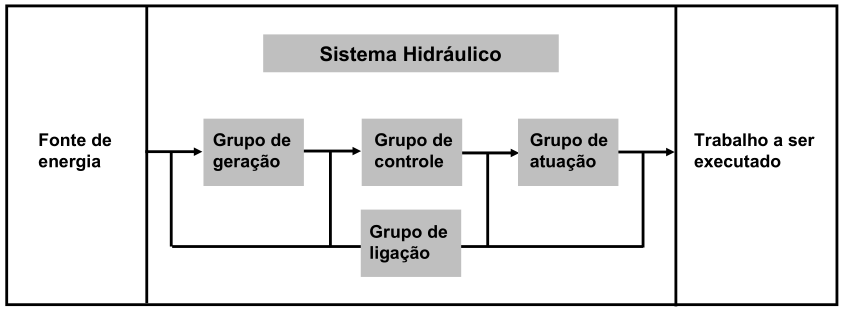
\includegraphics[width=0.7\linewidth]{Figuras/Ch15/fig7}

\end{frame}


\begin{frame}{Sistema hidráulico básico}
	\begin{block}{Fonte de energia - motores}
		\begin{itemize}
			\item Essa será a fonte de energia de todo o sistema.
		\end{itemize}
	\end{block}
	
	\centering
	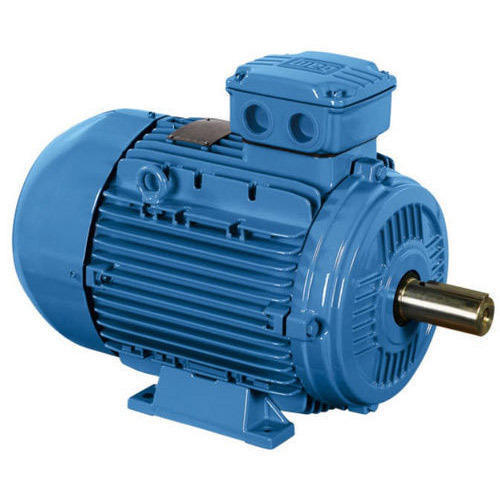
\includegraphics[width=0.55\linewidth]{Figuras/Ch15/fig8}
	
\end{frame}



\begin{frame}{Sistema hidráulico básico}
	\begin{block}{Grupo de geração - bombas hidráulicas}
		\begin{itemize}
			\item Assim como em pneumática, os fluidos hidráulicos precisam ser bombeados.
			\item As bombas mais comuns na hidráulica são as de \textbf{deslocamento positivo}.
		\end{itemize}
	\end{block}
	
	\centering
	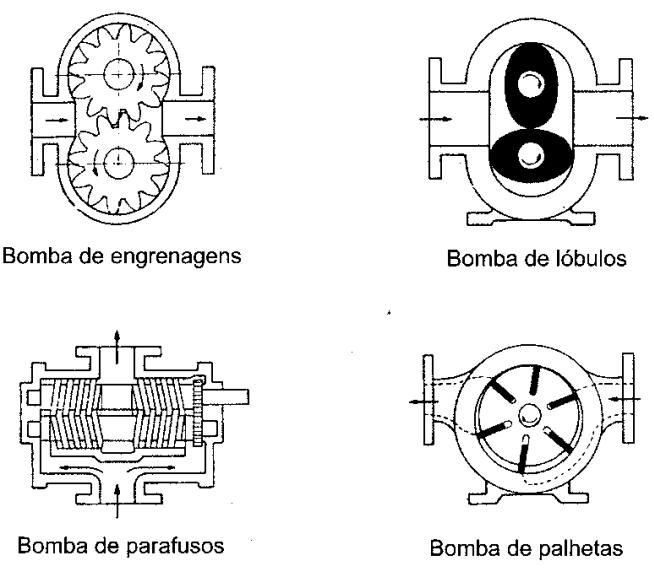
\includegraphics[width=0.45\linewidth]{Figuras/Ch15/fig5}
	
\end{frame}


\begin{frame}{Sistema hidráulico básico}

	\centering
	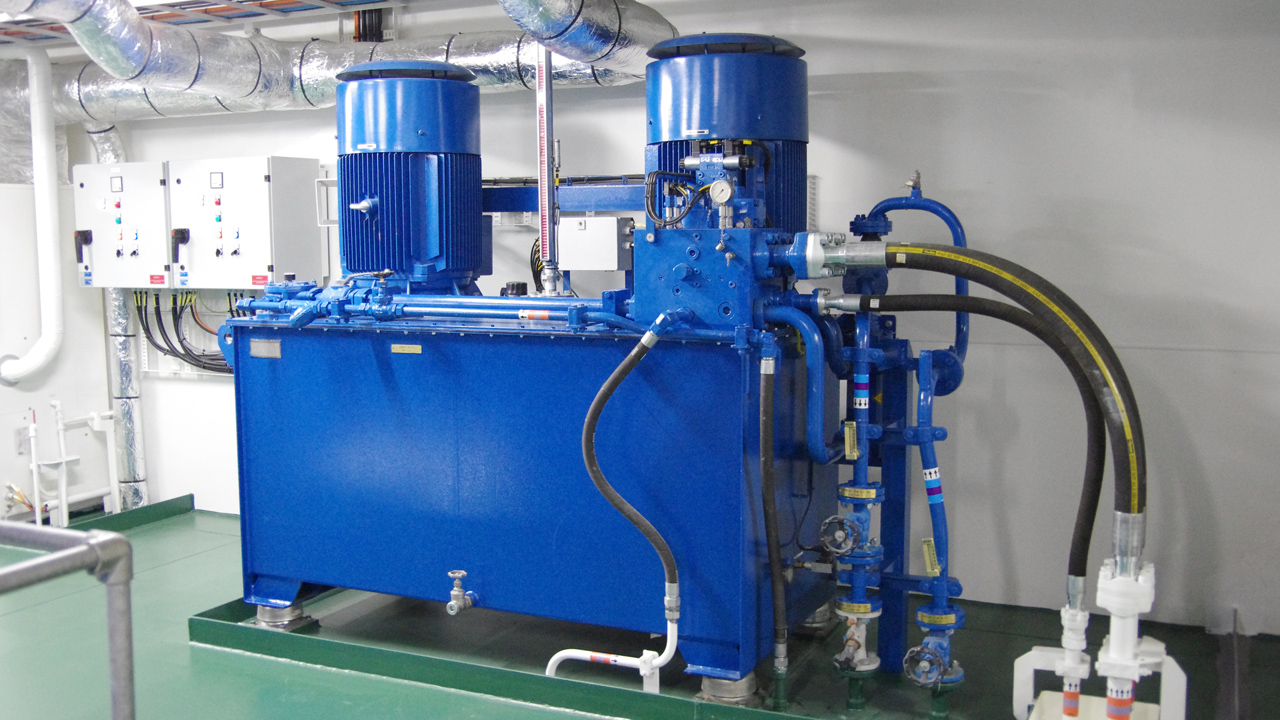
\includegraphics[width=0.9\linewidth]{Figuras/Ch15/fig9}
	
	\medskip
	
	Típica bancada para trabalho com fluido hidráulico
	
\end{frame}


\begin{frame}{Sistema hidráulico básico}
	\begin{block}{Grupo de controle - válvulas e comandos elétricos}
		\begin{itemize}
			\item Controla a potência hidráulica de forma similar a pneumática.
		\end{itemize}
	\end{block}

	\medskip
	
	\centering
	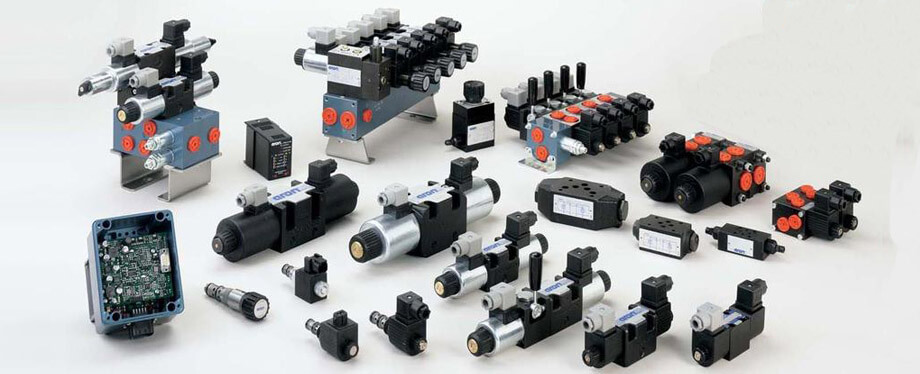
\includegraphics[width=0.8\linewidth]{Figuras/Ch15/fig10}
	
\end{frame}


\begin{frame}{Sistema hidráulico básico}
	\begin{block}{Grupo de atuação - cilindros e motores}
		\begin{itemize}
			\item Transforma potência hidráulica em mecânica.
		\end{itemize}
	\end{block}

	\medskip
	
	\centering
	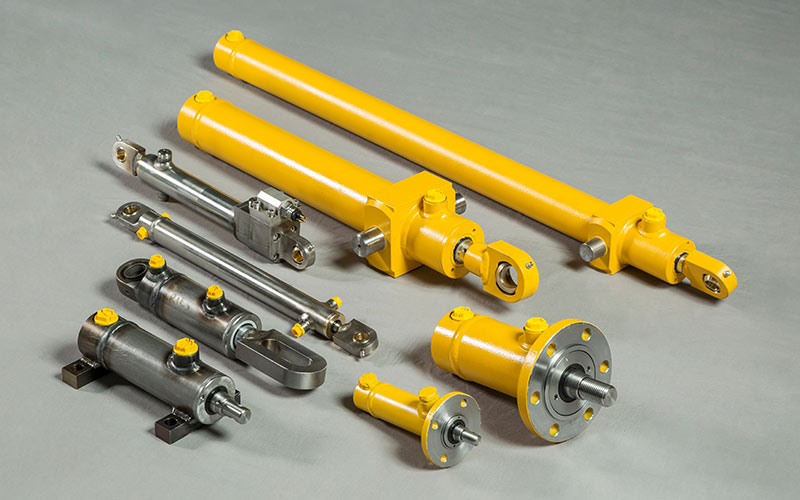
\includegraphics[width=0.7\linewidth]{Figuras/Ch15/fig11}
	
\end{frame}


\begin{frame}{Sistema hidráulico básico}
	\begin{block}{Grupo de ligação - conexões, tubos e mangueiras}
		\begin{itemize}
			\item Realizam o \textbf{transporte} do fluido de trabalho pelo sistema com \textbf{segurança} e \textbf{minimizando perdas}, além de \textbf{dissipar vibrações} do sistema.
		\end{itemize}
	\end{block}
	
	\medskip
	
	\centering
	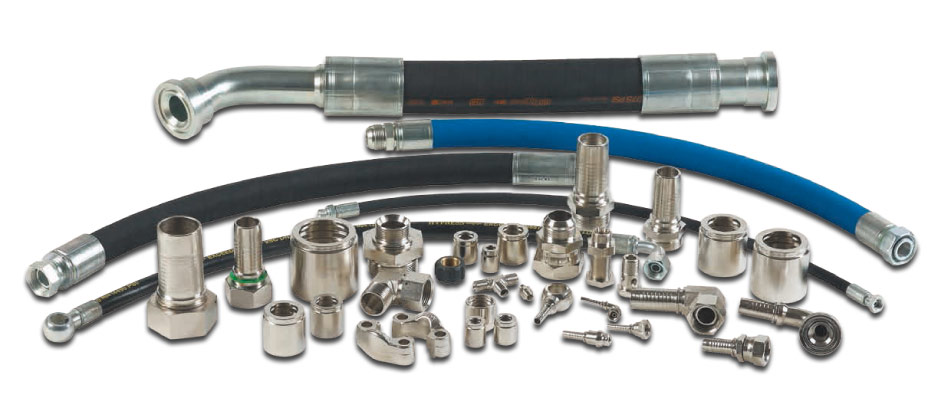
\includegraphics[width=0.9\linewidth]{Figuras/Ch15/fig12}
	
\end{frame}


\begin{frame}{Fluido hidráulico}
	\begin{block}{}
		O fluido hidráulico, apesar de não estar listado como componente do sistema básico hidráulico é \textbf{imprescindível} para o funcionamento de qualquer sistema desse tipo.
		
		\smallskip
		
		As quatro funções do fluido hidráulico num sistema são:
		\begin{itemize}
			\item Transmissão de energia.
			\item Lubrificação das partes móveis internas.
			\item Transferências de calor.
			\item Vedação de folgas entre partes móveis
		\end{itemize}
	\end{block}
\end{frame}


\begin{frame}{Fluido hidráulico}
	\begin{minipage}{.45\linewidth}
		\centering
		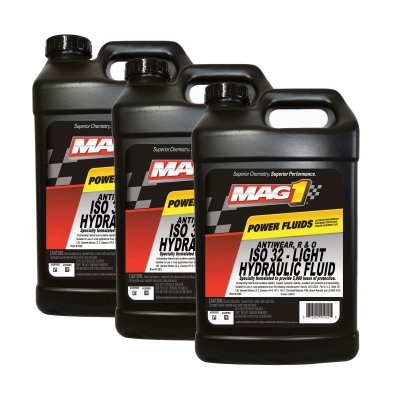
\includegraphics[width=1\linewidth]{Figuras/Ch15/fig13}
	\end{minipage}
	\hfill
	\begin{minipage}{.45\linewidth}
		\centering
		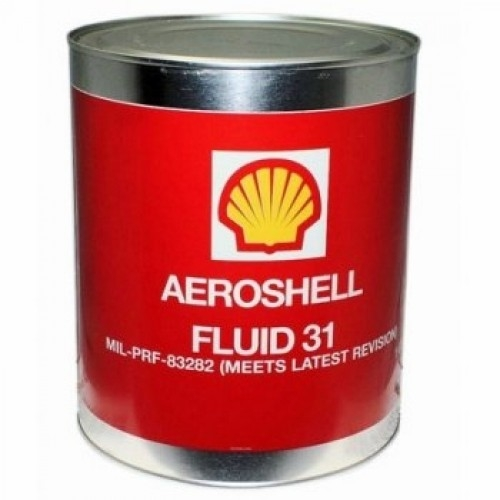
\includegraphics[width=1\linewidth]{Figuras/Ch15/fig14}
	\end{minipage}
\end{frame}


\begin{frame}{Filtragem}
	\begin{block}{Introdução}
		\textbf{Mais de 75\% das falhas em sistemas hidráulicos são devido ao excesso de contaminação.}
		
		\smallskip
		
		O excesso de contaminação provoca:
		\begin{itemize}
			\item Perda de produção.
			\item Custo de reposição de componentes.
			\item Trocas constantes de fluido.
			\item Custo no descarte do fluido.
			\item Aumento geral dos custos de manutenção.
		\end{itemize}
	\end{block}
\end{frame}


\begin{frame}{Filtragem}
	\begin{block}{}
		\begin{itemize}
			\item O maior problema na contaminação do fluido é sua interferência negativa na lubrificação.
			\item A falta de lubrificação causa \textbf{desgaste excessivo, resposta lenta, operações não-sequenciadas, queima da bobina do solenoide e falha prematura do componente}.
		\end{itemize}
	\end{block}

	\centering
	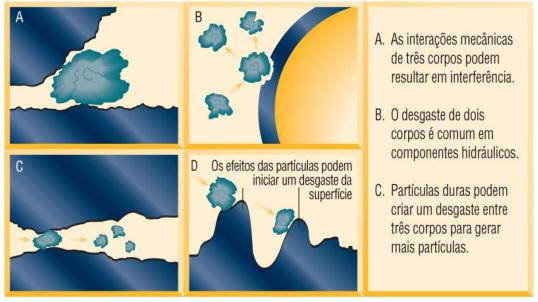
\includegraphics[width=0.7\linewidth]{Figuras/Ch15/fig15}
	
\end{frame}


\begin{frame}{Filtragem}
	\begin{block}{}
		\begin{itemize}
			\item Existem vários tipos de filtro de acordo com seu posicionamento no sistema hidráulico.
		\end{itemize}
	\end{block}

	\centering
	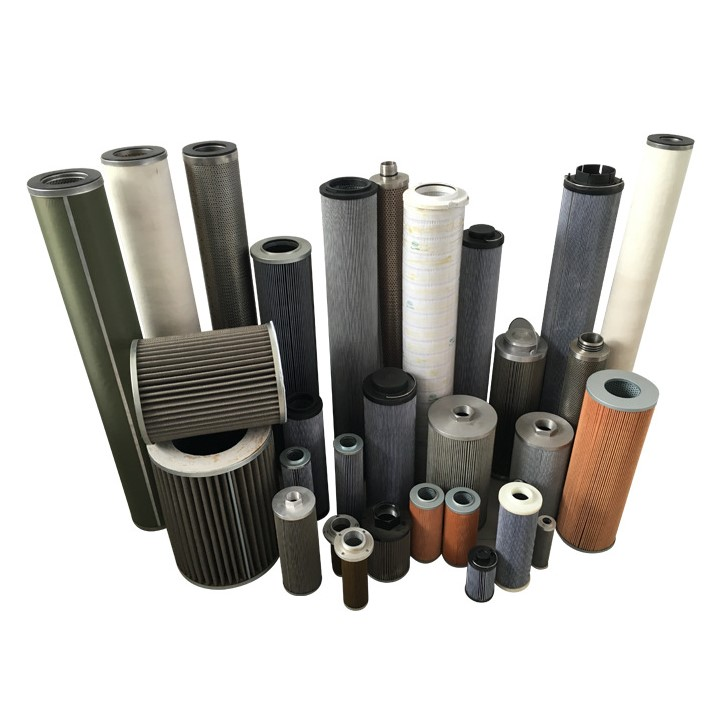
\includegraphics[width=0.6\linewidth]{Figuras/Ch15/fig16}

\end{frame}


\begin{frame}{Reservatório}
	\begin{block}{}
		\begin{itemize}
			\item O reservatório deve \textbf{guardar} todo o fluido hidráulico \textbf{em segurança}, recebendo-o após o \textit{loop} de utilização.
		\end{itemize}
	\end{block}

	\medskip
	
	\centering
	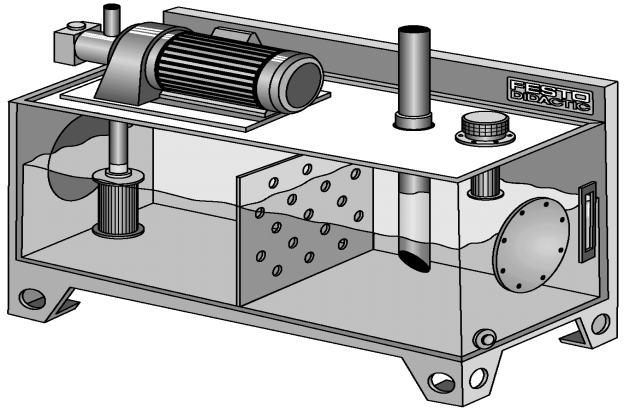
\includegraphics[width=0.6\linewidth]{Figuras/Ch15/fig17}
	
\end{frame}


\begin{frame}{Válvula redutora de pressão}
	\begin{block}{}
		\begin{itemize}
			\item Trata-se de uma \textbf{válvula de segurança}, que será atuada pela \textbf{pressão} do próprio \textbf{fluido de processo}.
			\item Como os motores usados na hidráulica tendem a causar \textbf{aumento de pressão} na linha, caso haja algum \textbf{bloqueio} nesta, há a possibilidade de \textbf{acidentes}.
			\item Para lidar com isso foram criadas as \textbf{válvulas redutoras}.
		\end{itemize}
	\end{block}

	\centering
	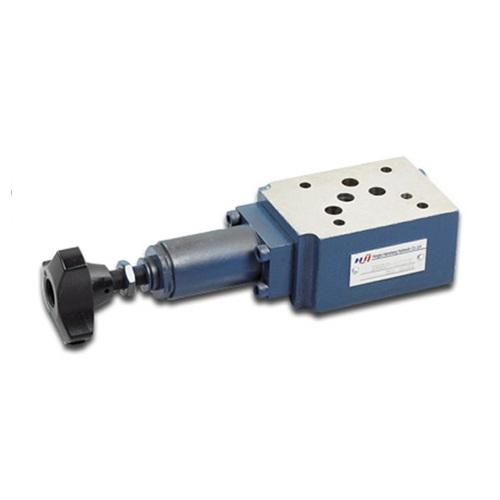
\includegraphics[width=0.45\linewidth]{Figuras/Ch15/fig18}
	
\end{frame}


\frame{
	\frametitle{Exercícios}
	\begin{block}{}
		01. Um guindaste precisa içar \num{230} toneladas em peso bruto de petróleo em um dia. Qual sistema será mais eficiente para essa aplicação (elétrico, pneumático ou hidráulico)? Explique.
		
		\vspace{0.5cm}
		
		02. Sabendo que um circuito hidráulico foi montado por um colega sem experiência, qual seria o primeiro ponto de falha a conferir antes de ligá-lo? Por quê?
	\end{block}
}

\section*{Referências}
\frame{
	\frametitle{Referências e Exercícios Complementares}
	\begin{itemize}
		\item MELCONIAN, Sarkis. Sistemas Fluidomecânicos - Hidráulica e Pneumática, 1 ed. Érica, 2014.
	\end{itemize}
	%\centering{\alert{Página 546 - \textbf{Capítulo 6}}} \\
	%\centering{\alert{Lista de exercícios 01}}
}
